\chapter{Hamilton-Jacobi equation}
\section{Derivation of the Hamilton-Jacobi equation}
In this final section regarding analytical mechanics we aim to prove and understand the so-called "Hamilton-Jacobi equation", which is the most abstract way of thinking about mechanics. Up to now we defined action as:
\begin{equation}
  S = \int_{t_1}^{t_2}\lagr\brackets{\vec{q},\dvec{q},t} \dd{t}
\end{equation}
Which means that we think about action as a functional. Now we want to express the same quantity as a function of time and to do so, we need to slightly change our definition:
\begin{equation}
  S \defineeq \int_{t_0}^{t}\lagr\brackets{\vec{q},\dvec{q},t} \dd{t}
\end{equation}
We need to remember that the integral of action \underline{must} be calulated along the actual path of the system we are dealing with, but with this definition, in principle, we can obtain $S$ as a function of time. In particular, we want to prove that $S$ is a function of both time and all the $q_{\alpha}$.
\begin{proof}
  The proof for the time dependence is trivial since:
  \begin{equation}
    \dv{S}{t} = \lagr
  \end{equation}
  For the dependence on $q_{\alpha}$ we can imagine to chang the coordinates without changing the actual path and the time:
  \begin{figure}[H]
    \centering
    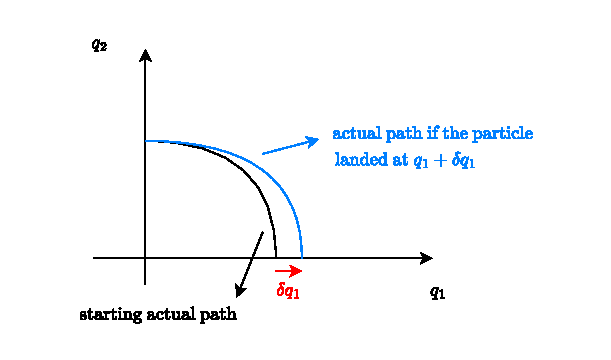
\includegraphics[width=0.6\textwidth]{res/svg/path_change_hamjac.drawio}
    \caption{Path change}
\end{figure}
How does $S$ change for the two trajectories?
\begin{equation}
  \delta S = \int_{t_0}^{t}\cancel{\bigsum_{\alpha}\brackets{\pdv{\lagr}{q_{\alpha}}-\dv{}{t}\pdv{\lagr}{\dot{q}_{\alpha}}}}\delta q_{\alpha} + \int_{t_0}^{t} \dv{}{t} \brackets{\bigsum_{\alpha} \pdv{\lagr}{\dot{q}_{\alpha}}\delta q_{\alpha}}
\end{equation}
We cancel the first part since when we are integrating over the actual path the \eleref\;are true. We then get:
\begin{equation}
  \begin{split}
    \delta S &= \int_{t_0}^{t}\dv{}{t}\brackets{\bigsum_{\alpha} \pdv{\lagr}{\dot{q}_{\alpha}}\delta q_{\alpha}}\\
    &= \bigsum_{\alpha} \pdv{\lagr}{\dot{q}_{\alpha}}\delta q_{\alpha}\bigg|_{t_0}^t =\\
    &= \bigsum_{\alpha} \pdv{\lagr(t)}{\dot{q}_{\alpha}}\delta q_{\alpha}(t) =\\
    &= \bigsum_{\alpha} p_{\alpha} \dd{q_{\alpha}}
  \end{split}
\end{equation}
When we evaluate at $t_0$ the variation is zero since the extremes are fixed. From the final result we have that:
\begin{equation}
  \pdv{S}{q_{\alpha}} = p_{\alpha}
\end{equation}
And so $S$ depends on $q_{alpha}$
\end{proof}

